\newpage
\section{Управление движением робота}
\subsection{Кинематическая модель}
Кинематическая модель робота имеет вид~\cite{survey}:
\begin{equation}\label{eq_robot_kinematic_model}
    \left\{
    \begin{aligned}
        & \dot{x} = v \cos \theta \\
        & \dot{y} = v \sin \theta \\
        & \dot{\theta} = \omega
    \end{aligned}
    \right.
\end{equation}
где $x$, $y$~--- декартовы координаты точки~$C$, являющейся серединой задней оси (см.~рисунок~\ref{img_kinematic_model_picture}); $\theta$~--- угол поворота робота (угол между осями абсцисс неподвижной системы координат $Ox_0y_0$ и системы координат $Ox_1y_1$, жёстко связанной с роботом); $v$~--- проекция скорости~$\vec{v}$ точки~$C$ на ось абсцисс системы координат~$Ox_1y_1$\!\footnote{В~данной работе проскальзывание задних колес робота считается отсутствующим, а, следовательно, вектор $\vec{v}$~--- всегда коллинеарным оси абсцисс системы координат~$Ox_1y_1$.}; $\omega$~--- угловая скорость вращения робота.

\begin{figure}[h]
    \centering
    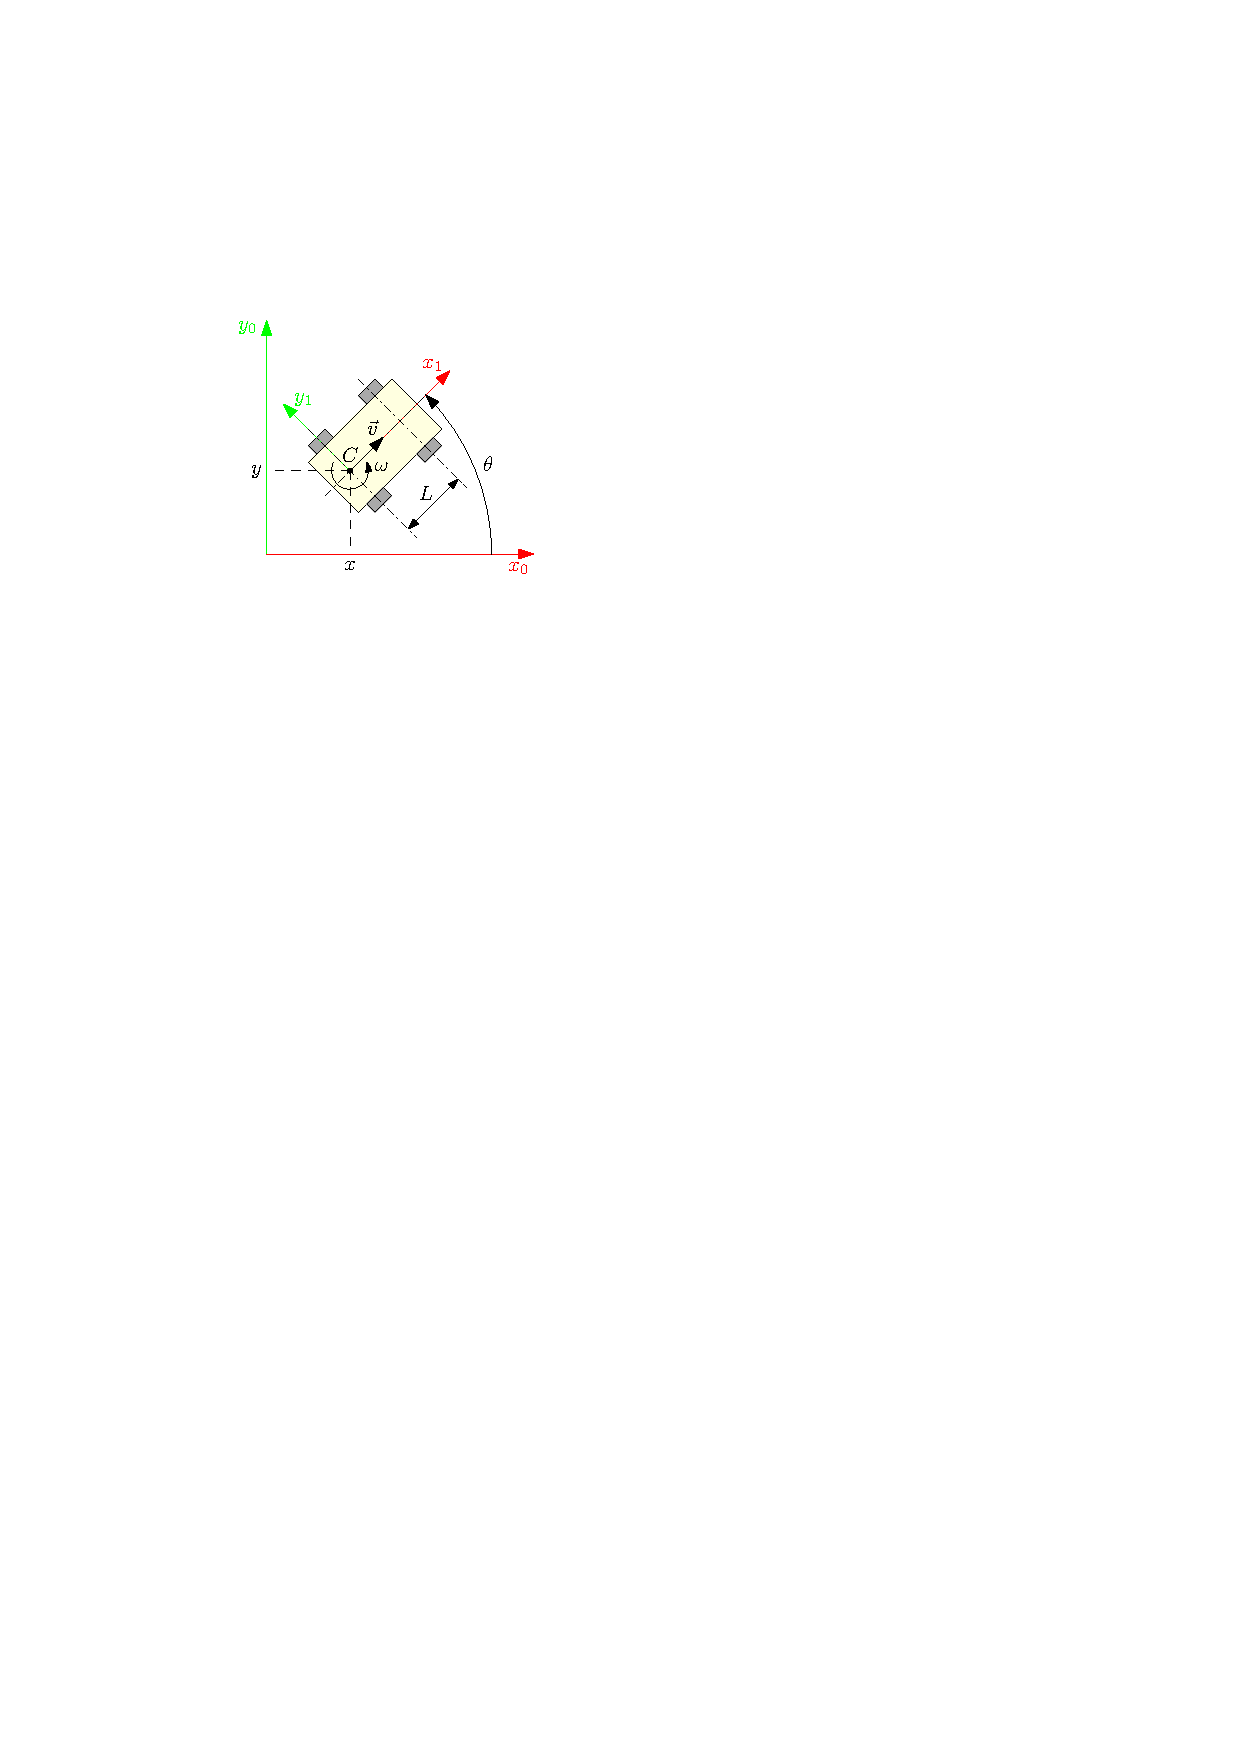
\includegraphics[width=0.5\textwidth]{kinematic_model_picture.pdf}
    \caption{Чертеж-пояснение к кинематической модели робота.}
    \label{img_kinematic_model_picture}
\end{figure}

Угловая скорость $\omega$ для робота-машинки с одним поворотным колесом оказывается связанной с углом его поворота~$\varphi$ выражением~\cite{survey}
\begin{equation}\label{eq_omega_of_phi}
    \omega = \frac{v}{L} \tg\varphi\ldotp
\end{equation}
Это равенство получается объединением следующих двух уравнений:
\begin{gather}
    \omega = \frac{v}{R}, \\
    \tg\varphi = \frac{L}{R} \label{eq_tg_phi},
\end{gather}
где $R$~--- радиус дуги, по которой двигается робот, а точнее точка $C$ (см.~рисунок~\ref{img_one_wheel_robot}).

\begin{figure}[h]
    \centering
    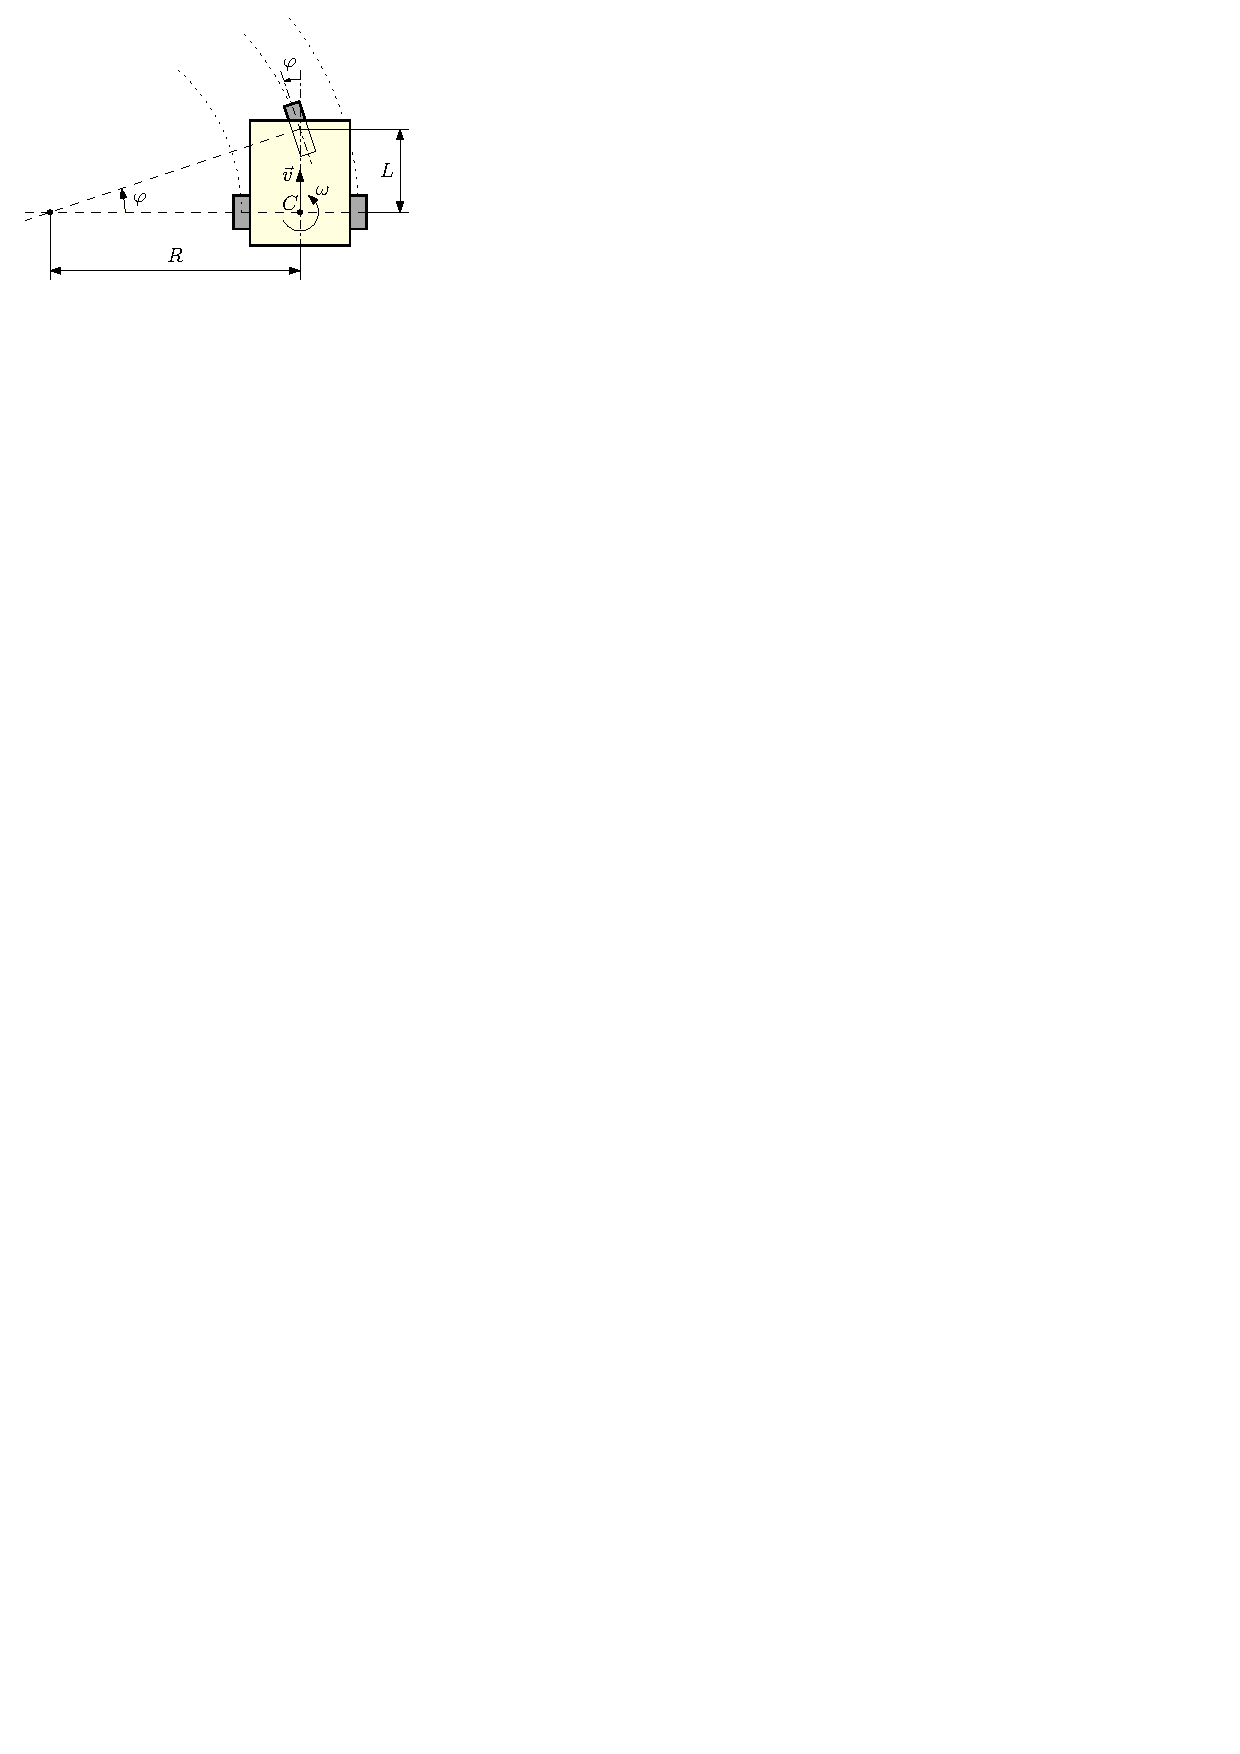
\includegraphics[width=0.5\textwidth]{one_wheel_robot.pdf}
    \caption{Движение робота с одним рулевым колесом по дуге.}
    \vspace{0cm}
    \label{img_one_wheel_robot}
\end{figure}

Так как у робота из данной работы колеса два, и примененная в нем рулевая трапеция не обеспечивает их точного поворота на те углы, при которых они не будут проскальзывать в поперечном направлении~\cite{ackerman_steering}, использование по отношению к нему выражений~\eqref{eq_omega_of_phi}--\eqref{eq_tg_phi}, строго говоря, невозможно.
При этом с ожиданием получения от нее приближенных, но близких к истинным результатов расчетов первое из этих выражений в форме
\begin{equation}
    \omega = \frac{v}{L} \tg \bar\varphi \ldotp
\end{equation}
где $\bar\varphi$~--- угол поворота вала рулевого двигателя, все же используется в данной работе.
Основанием этого решения являются результаты <<моделирования>> работы рулевой трапеции в программе GeoGebra (см.~рисунок~\ref{img_steering_geogebra}), согласно которым перпендикуляры к передним колесам и  поворотному коромыслу не пересекаются на прямой, проходящей через ось вращения задних колес, совсем немного.

\begin{figure}[h]
    \centering
    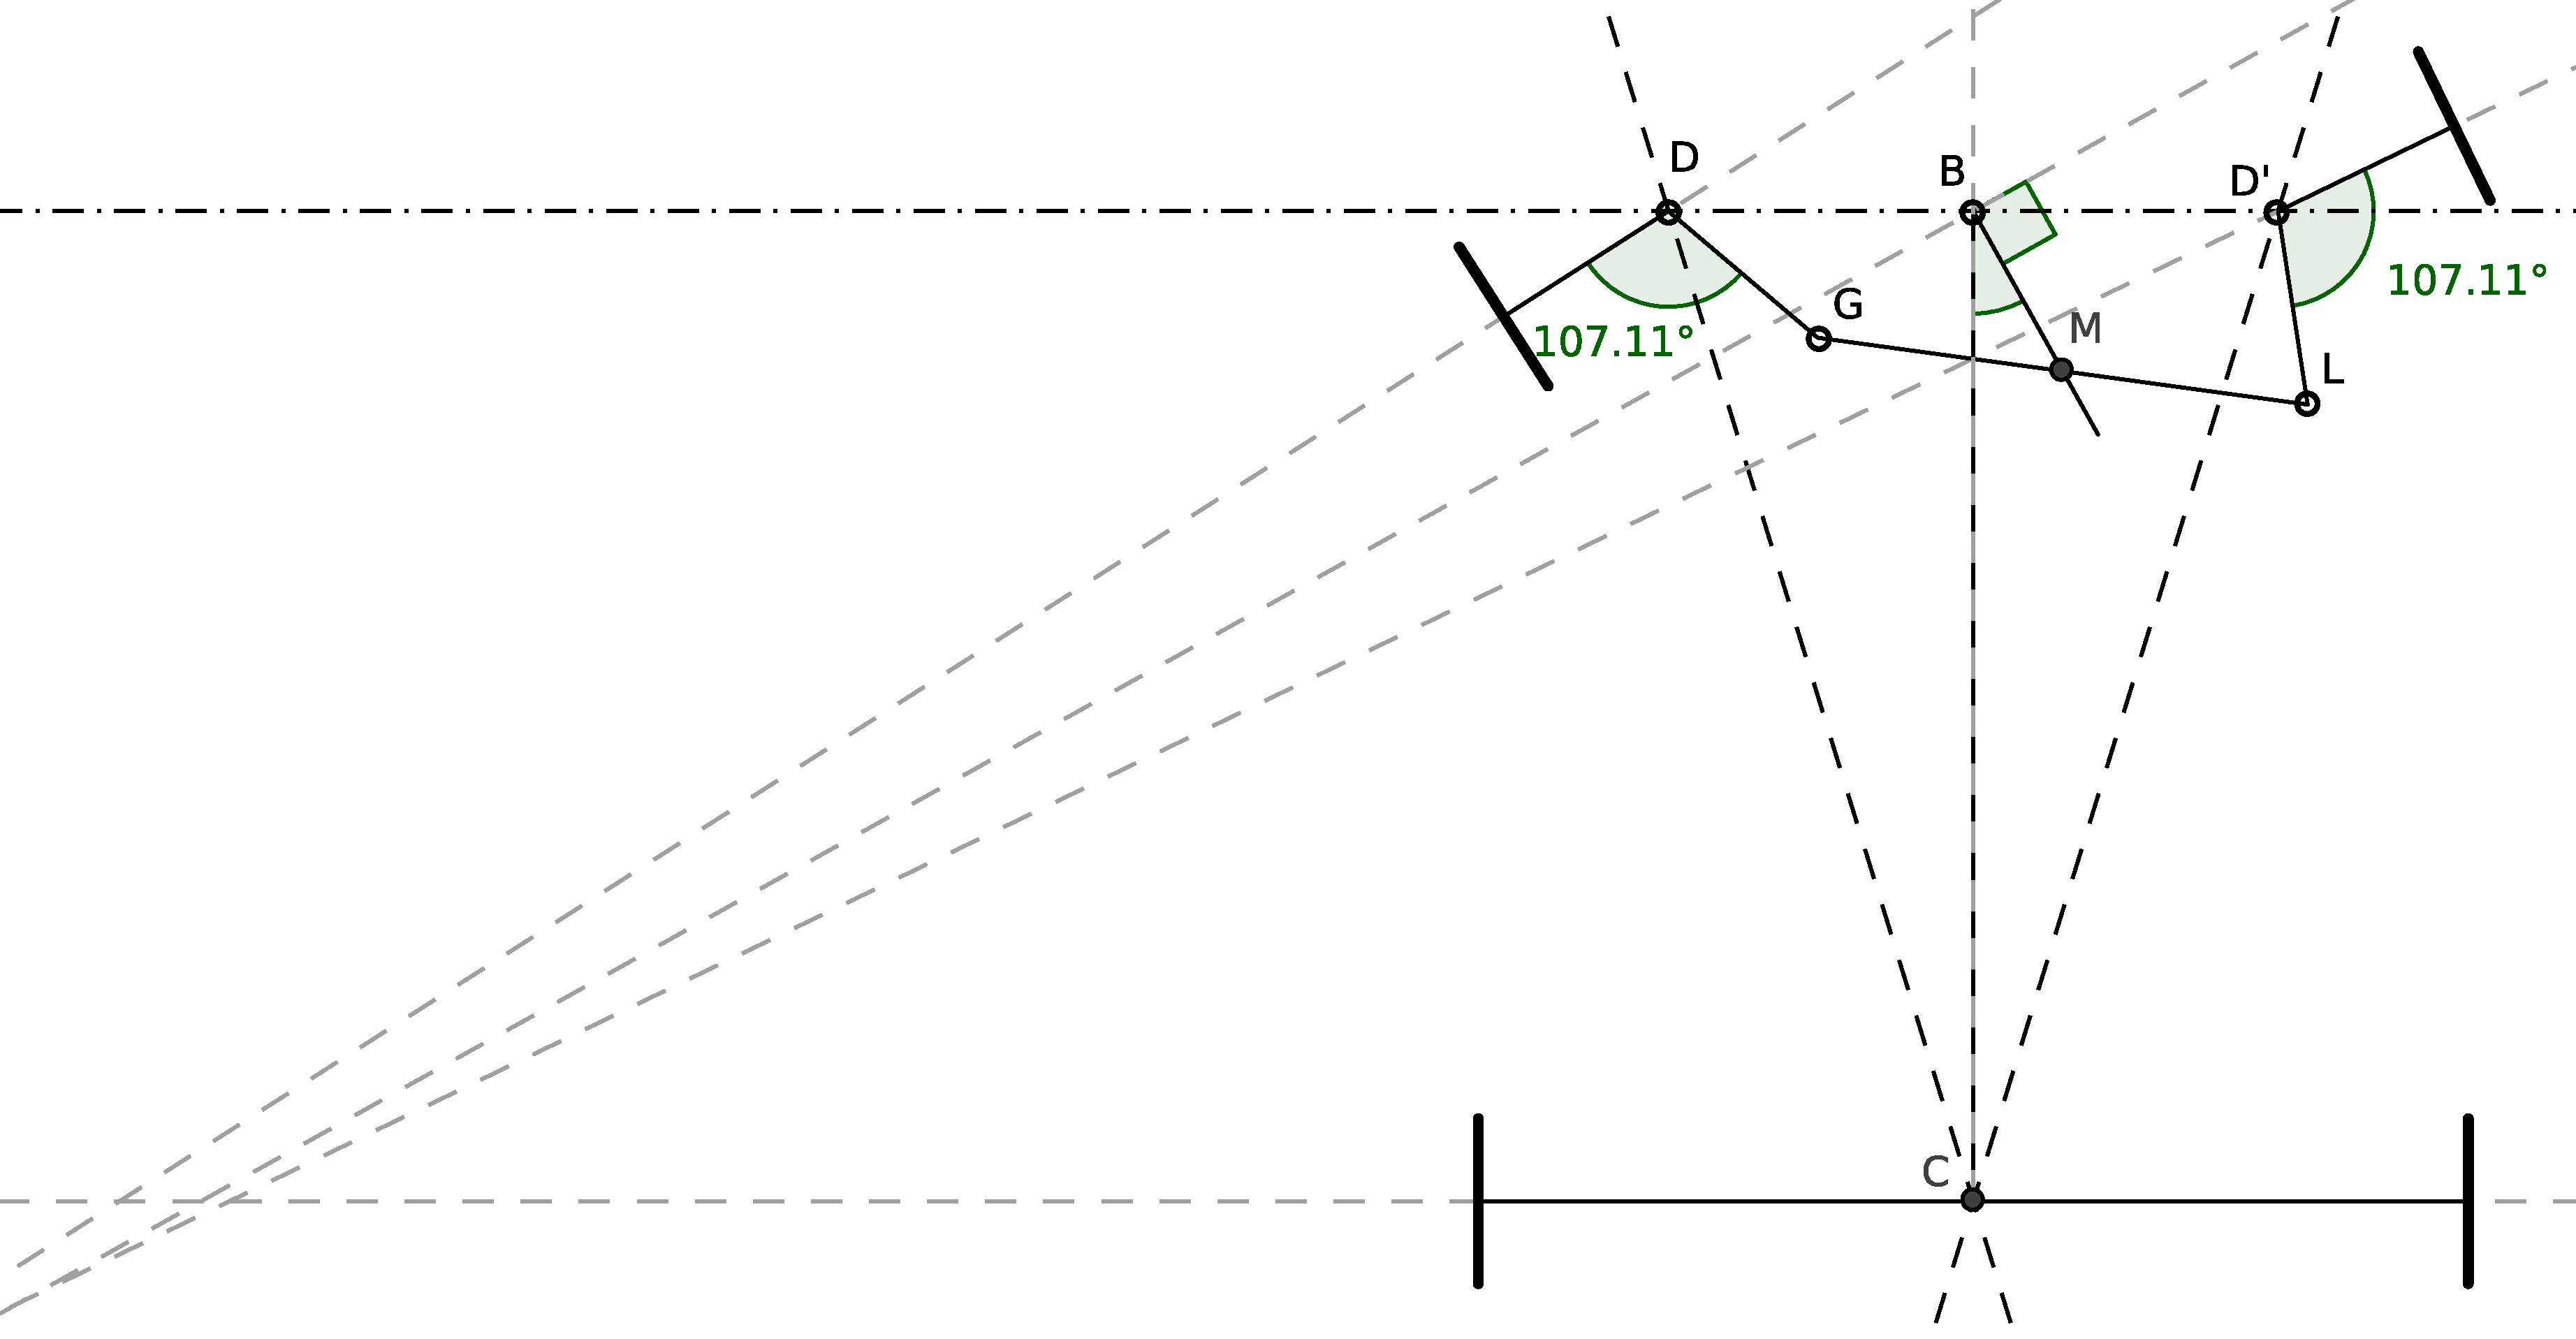
\includegraphics[width=0.9\textwidth]{steering_geogebra.pdf}
    \caption{Рулевая трапеция в смещенном относительно центрального положении ($\angle CBM = \bar{\varphi}$, $GM=ML$, $|BM|=var$).}
    \vspace{0cm}
    \label{img_steering_geogebra}
\end{figure}



\subsection{Локализация робота}
В~качестве угла~$\theta$ и угловой скорости~$\omega$ в работе использовались угол и угловая скорость, возвращаемые установленным на робота датчиком-гироскопом.
Координаты $x$ и $y$, в свою очередь, непосредственно не измерялись, а рассчитывались с использованием первых двух уравнений модели~\eqref{eq_robot_kinematic_model}.
При этом линейная скорость точки~$C$ с учетом третьего пункта перечня, представленного в разделе~\ref{part_robot_features}, определялась в соответствии со следующим выражением
\begin{equation}
    v = \underline{\omega} r,
\end{equation}
где $\underline{\omega}$~--- угловая скорость вращения вала тягового двигателя, $r$~--- радиус задних колес робота.

Состоятельность описанного принципа локализации робота была проверена с помощью сторонней системы технического зрения.
Подробности соответствующих экспериментов и полученные результаты доступны в Приложении~\ref{app_cv_system}.



\subsection{Структура системы управления}
Общая структура системы управления движением робота, позволяющая ему двигаться по желаемой траектории, показана на рисунке~\ref{img_control_system}.
Указанные на ней физические величины, ранее не упоминавшиеся в тексте данного отчета, значат следующее:
\begin{ESKDexplanation}
    \item $U_1$ ($U_2$)~--- напряжение, подаваемое на тяговый (рулевой) двигатель, выраженное в процентах от максимального напряжения (знак определяет направление вращения);
    \item $\bar\varphi$~--- угол поворота вала рулевого двигателя;
    \item $\bar{\varphi}_{min}$, $\bar{\varphi}_{max}$~--- его минимальное и максимальное значения ($\bar{\varphi}_{min} = -\bar{\varphi}_{max}$);
    \item $x_r$ и $y_r$~--- координаты, которые должен иметь робот в данный момент времени, чтобы следовать по желаемой траектории;
    \item $X_{des}$~--- желаемое значение величины~$X$.
\end{ESKDexplanation}

\begin{figure}[h]
    \centering
    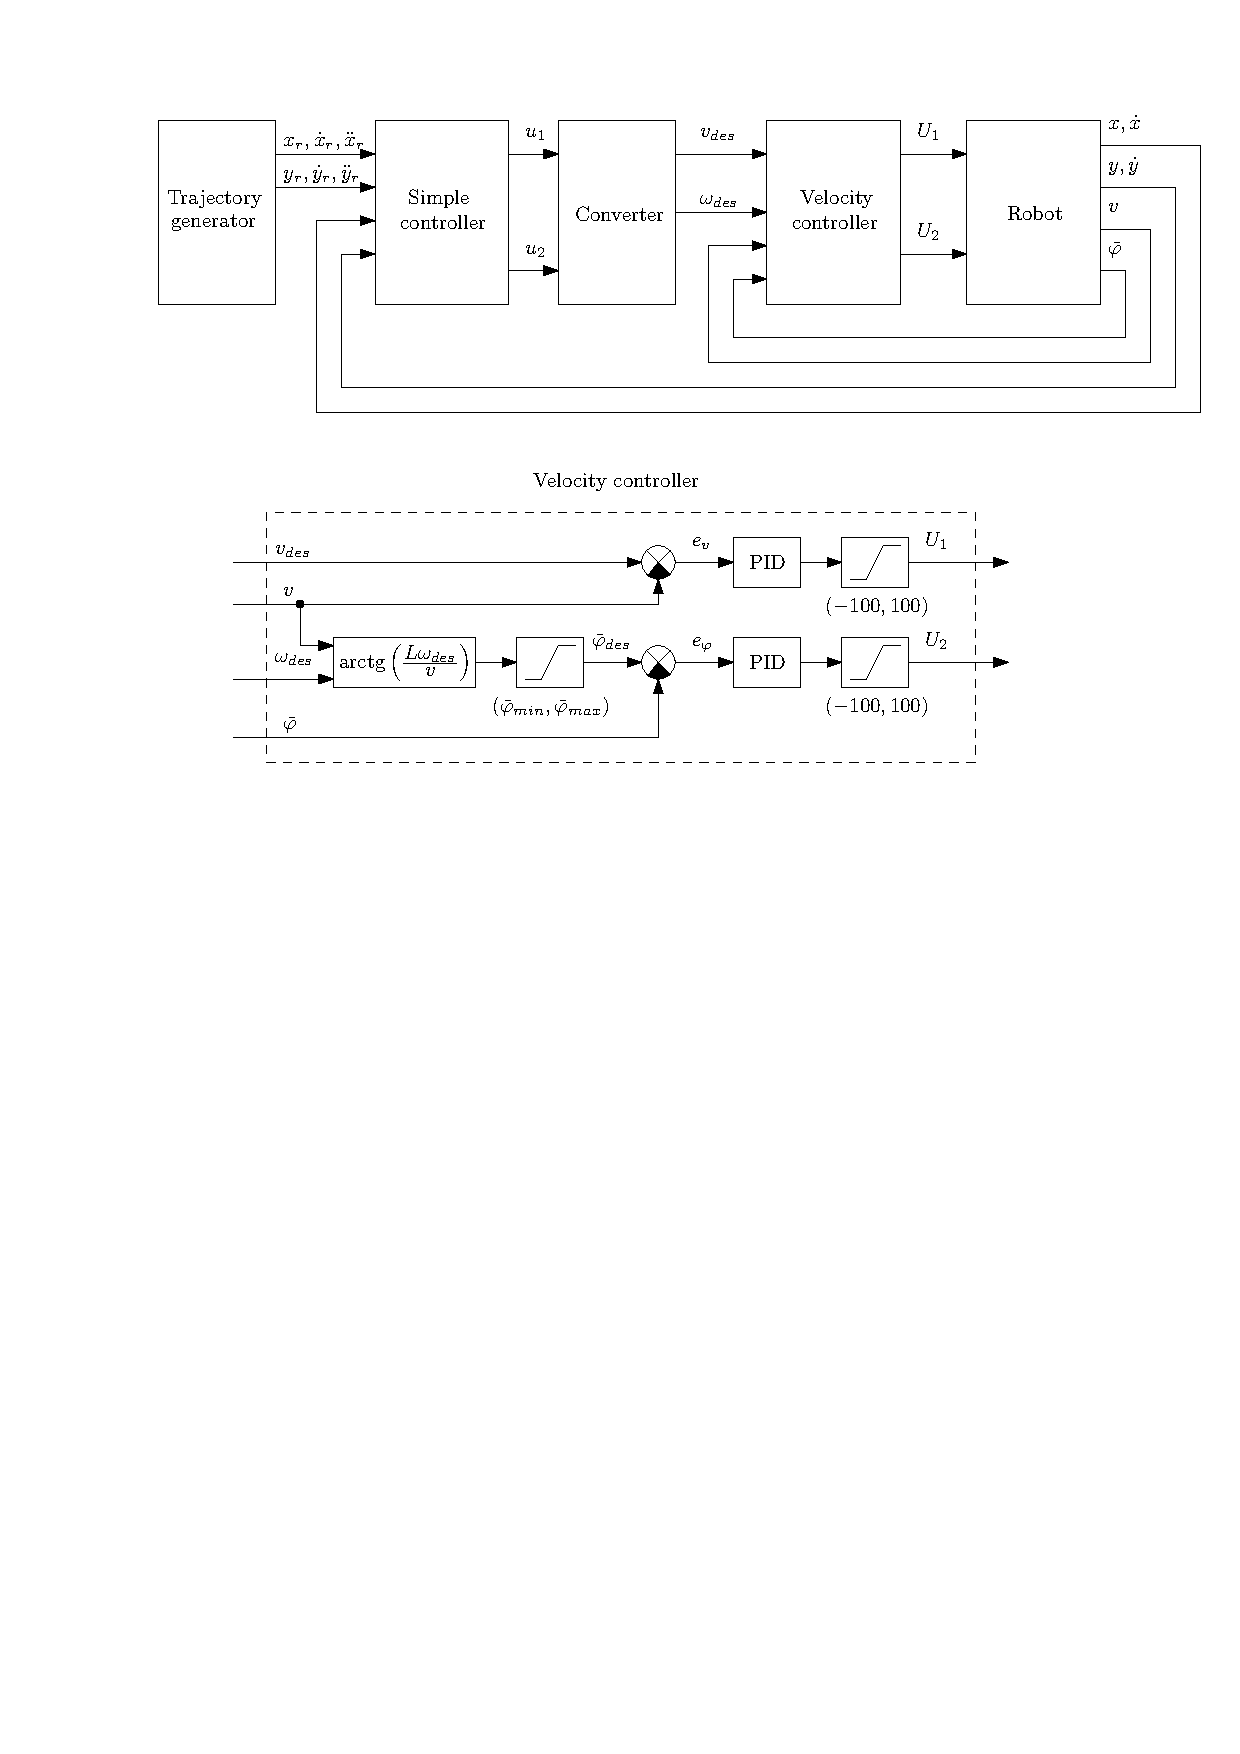
\includegraphics[width=\textwidth]{control_system.pdf}
    \vspace{0.0cm}
    \caption{Структура системы управления движением робота.}
    \label{img_control_system}
\end{figure}

Входящие в блок Velocity Controller ПИД-регуляторы были настроены вручную.
Качество их работы можно оценить из переходных функций, показанных на рисунках~\ref{img_v_pid} и~\ref{img_phi_pid}.

Качество управления угловой скоростью по прямой связи, включающей в себя функцию $\arctg()$, можно оценить из рисунка~\ref{img_angular_speed_feedworward}.

Формирование желаемых значений для линейной и угловой скоростей робота блоком Converter, а также расчет <<предварительных>> управляющих воздействий в блоке Simple Controller производятся в соответствии со следующими выражениями~\cite{de_luca}:
\begin{gather}
    \left\{
    \begin{aligned}
        & \dot{\xi} = u_1 \cos \theta + u_2 \sin \theta, \\
        & v_{des} = \xi, \\
        & \omega_{des} = \frac{-u_1 \sin \theta + u_2 \cos \theta}{\bar\xi},
    \end{aligned}
    \right.
    \qquad
    \bar\xi =
    \begin{cases}
        -0.01, & 0 > \xi \ge -0.01 \\
        0.01, & 0 \leqslant \xi \leqslant 0.01 \\
        \xi, & \text{иначе}
    \end{cases}
    \\
    \left\{
    \begin{aligned}
        & u_1 = \ddot{x}_r + k_{p1} (x_r - x) + k_{d1} (\dot{x}_r - \dot{x}), \\
        & u_2 = \ddot{y}_r + k_{p2} (y_r - y) + k_{d2} (\dot{y}_r - \dot{y})\ldotp
    \end{aligned}
    \right.
\end{gather}

Результаты запуска схемы моделирования, показанной на рисунке~\ref{img_control_system_modeling_scheme}\lefteqn{,}\footnote{В данной схеме в качестве модели робота-машинки использована модель~\eqref{eq_robot_kinematic_model}. Другими словами, блок Velocity Controller опущен <<за ненадобностью>>, и $v_{des} = v$,  $\omega_{des} = \omega$.} свидетельствуют о надлежащем функционировании этой системы управления (см.~рисунок~\ref{img_simulation_trajectory}).
В~условиях же реальных экспериментов она показала себя неработоспособной (см.~рисунок~\ref{img_movement_experiments_results}).

\begin{figure}[h!]
    \centering{ 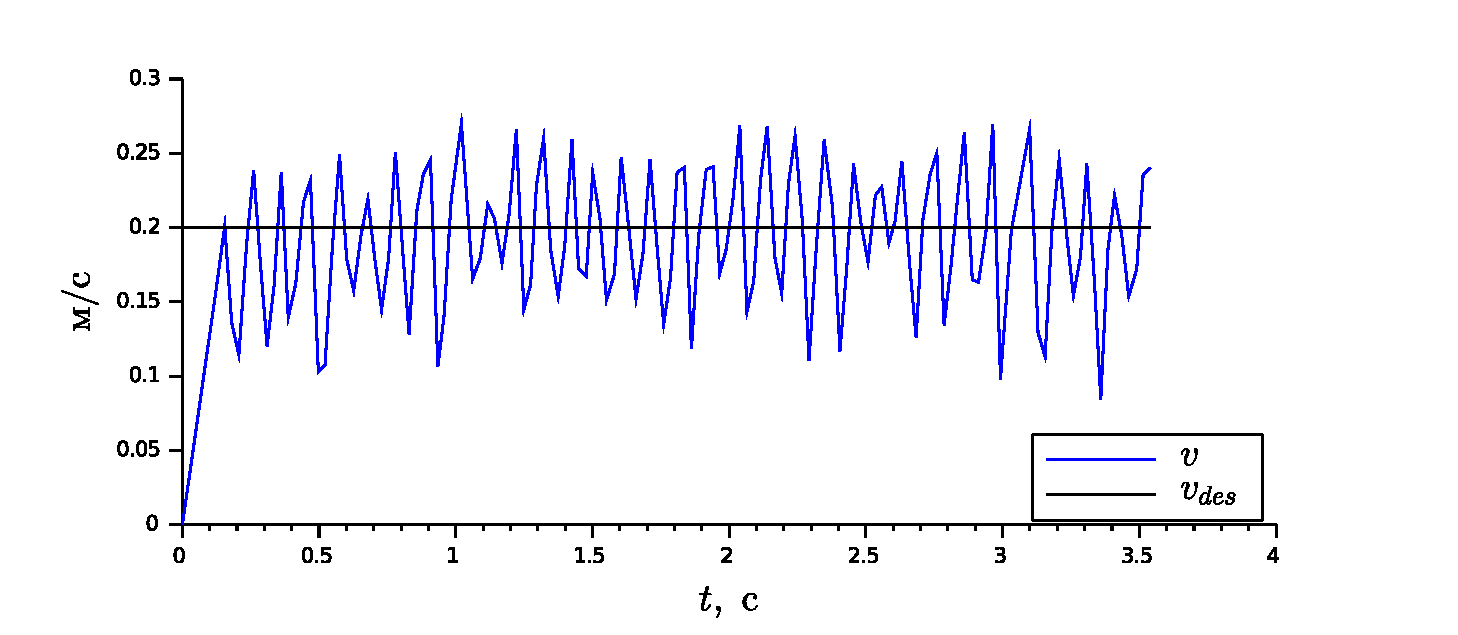
\includegraphics[width=\textwidth]{lin_vel_ht_1.pdf} \\ a) \\}
    \centering{ 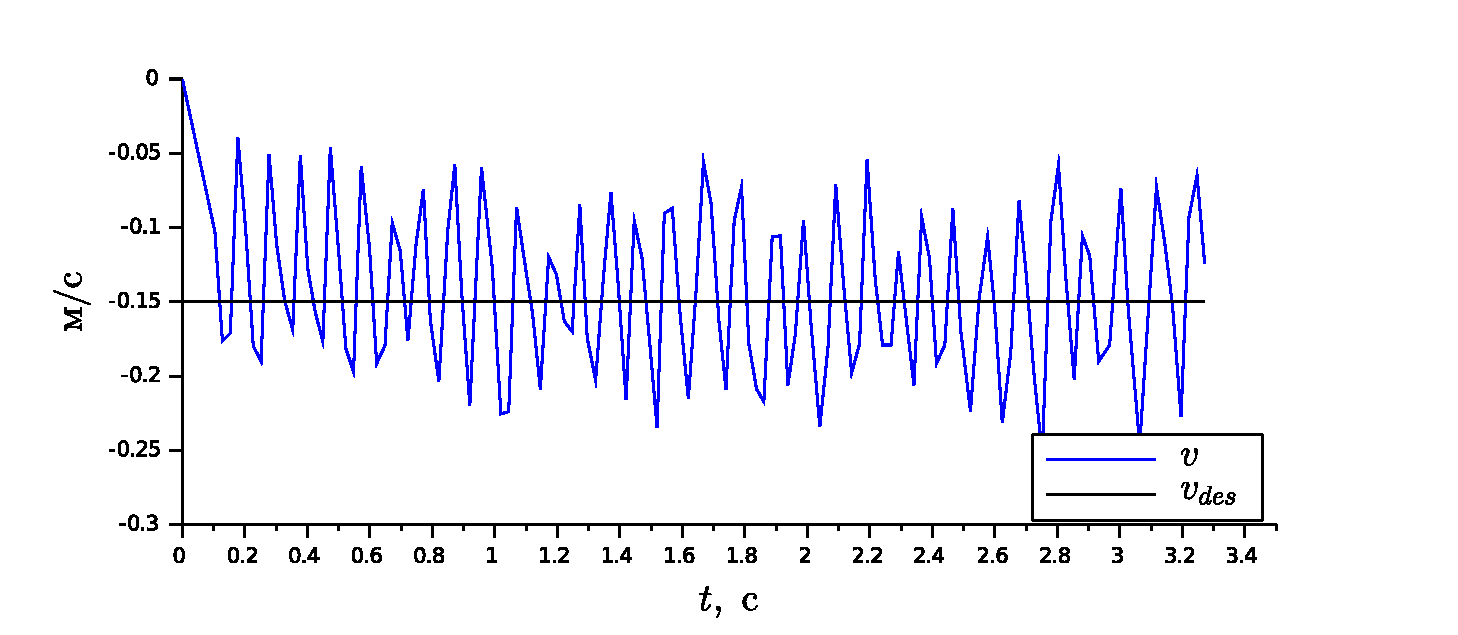
\includegraphics[width=\textwidth]{lin_vel_ht_2.pdf} \\ б) }
    \caption{Переходные функции ПИД-регулятора, управляющего значением скорости~$v$: a~--- при $v_{des} > 0$, б~--- при $v_{des} < 0$.}
    \label{img_v_pid}
\end{figure}

\begin{figure}[h!]
    \centering{ 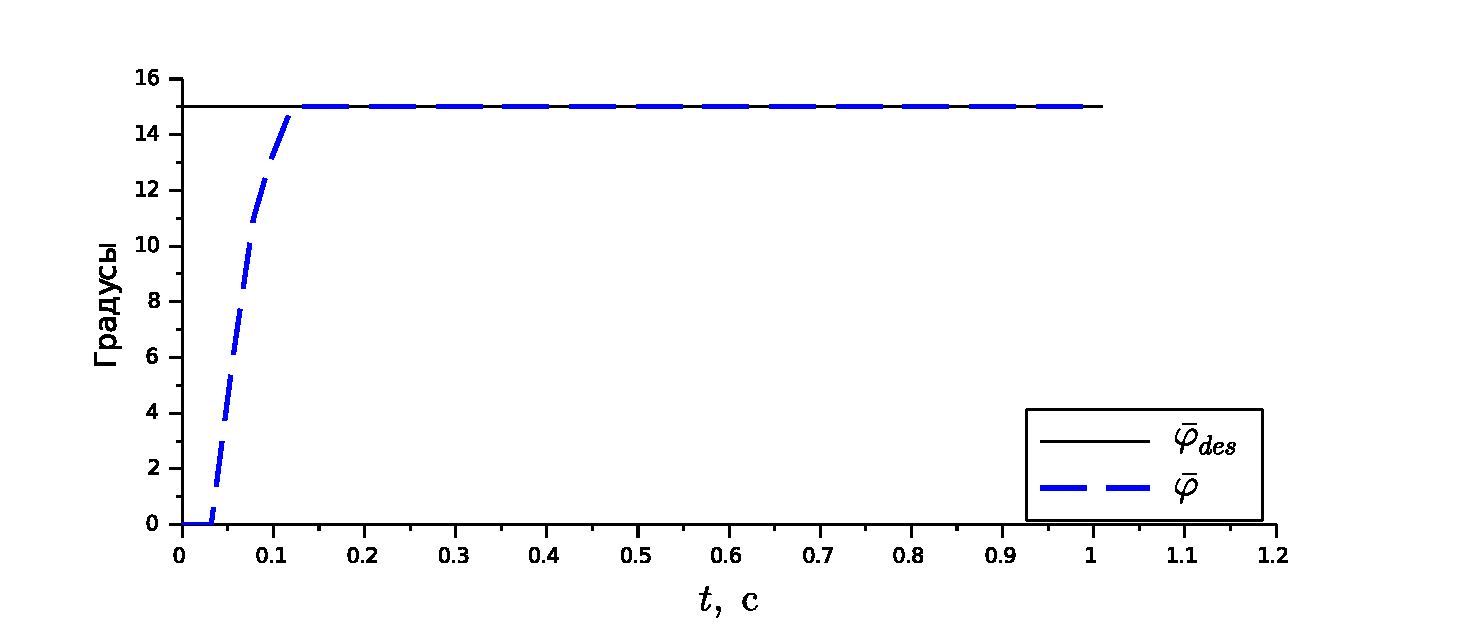
\includegraphics[width=\textwidth]{phi_ht_1.pdf} \\ a) \\}
    \centering{ 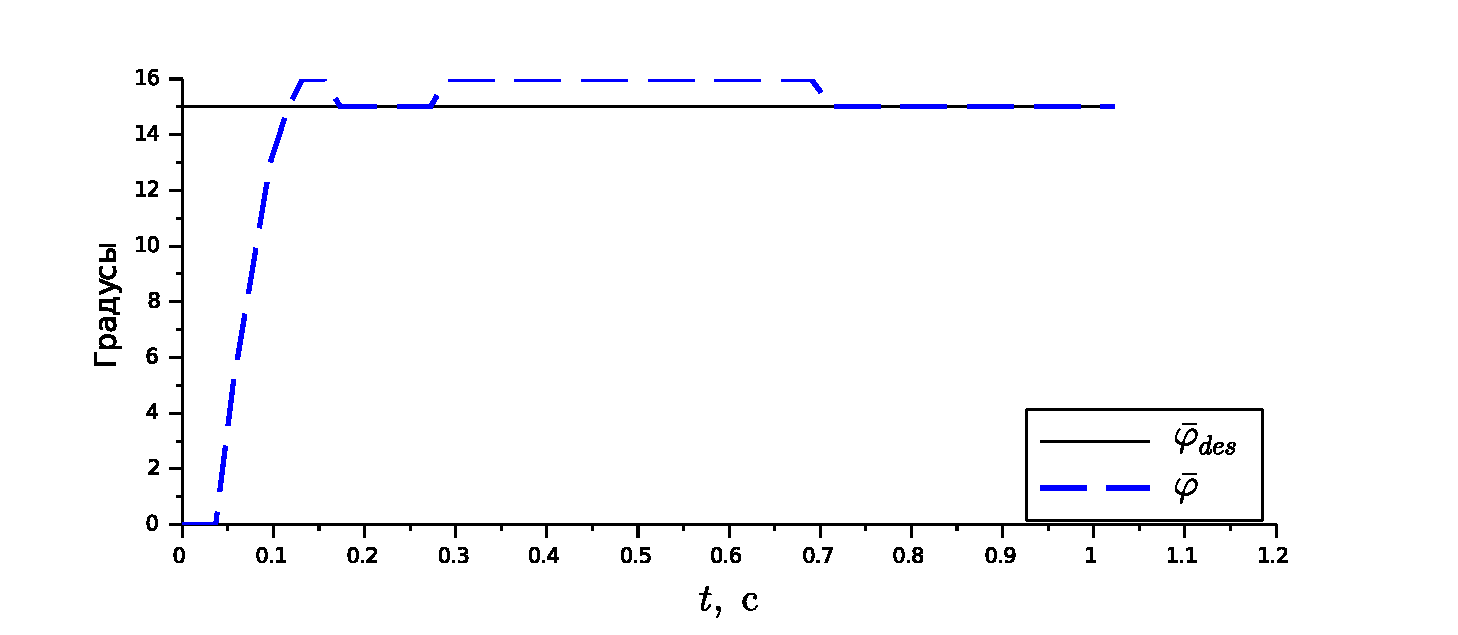
\includegraphics[width=\textwidth]{phi_ht_2.pdf} \\ б) }
    \caption{Переходные функции ПИД-регулятора, управляющего значением угла~$\bar{\varphi}$:\\ а~--- при $v = 0$, б~--- при $v \ne 0$.}
    \label{img_phi_pid}
\end{figure}

\begin{figure}[h!]
    \centering{ 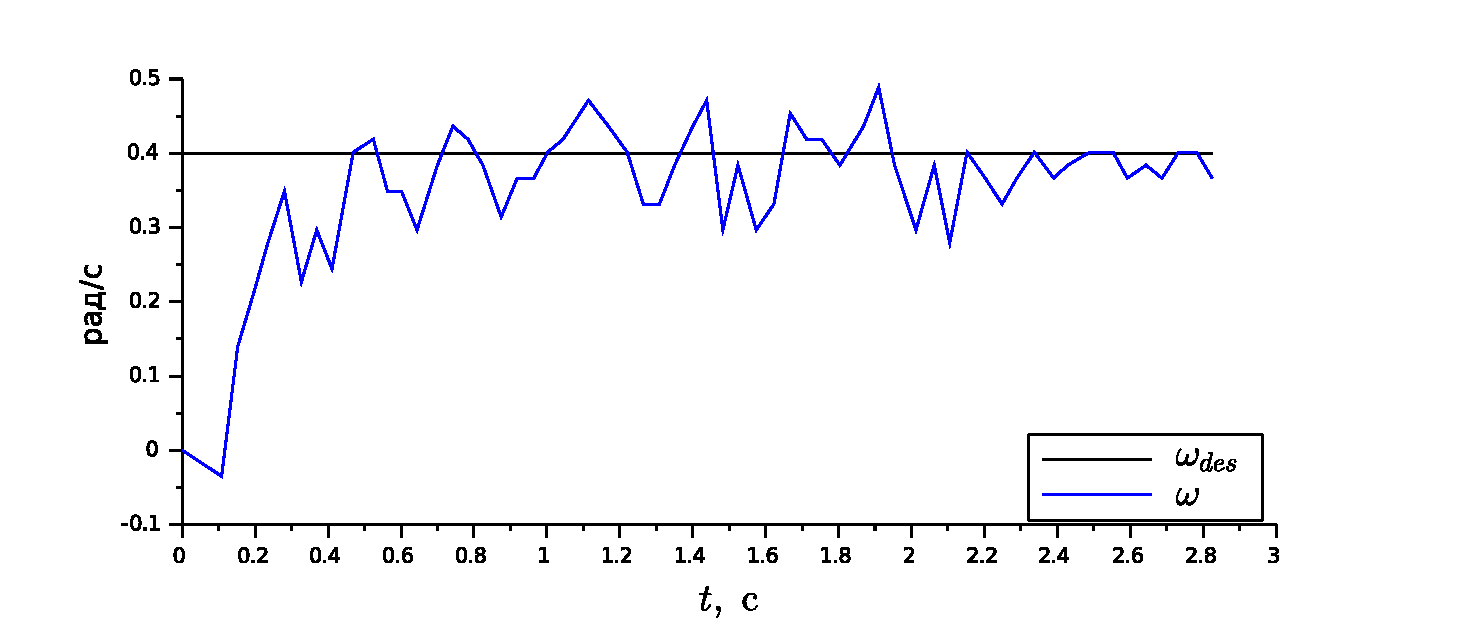
\includegraphics[width=\textwidth]{ang_vel_ht_1.pdf} \\ a) \\}
    \centering{ 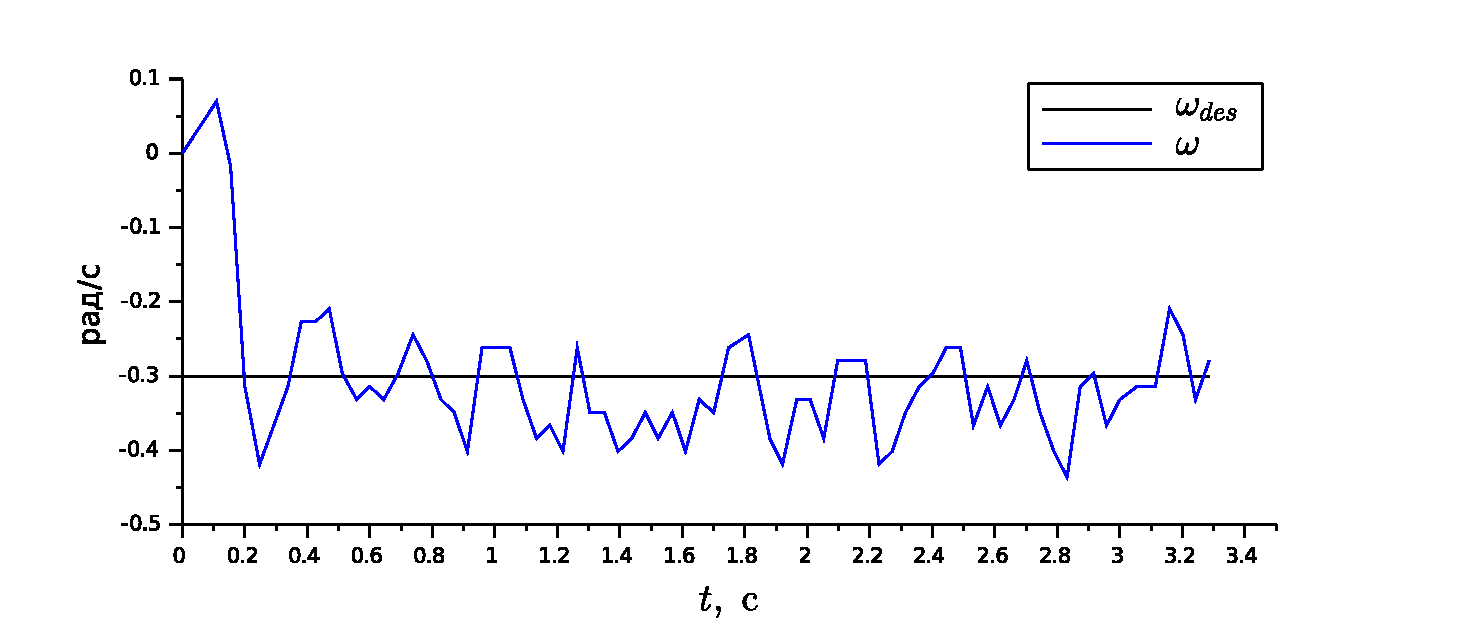
\includegraphics[width=\textwidth]{ang_vel_ht_2.pdf} \\ б) }
    \vspace{0.0cm}
    \caption{Переходные функции системы управления угловой скоростью.}
    \label{img_angular_speed_feedworward}
\end{figure}

\begin{figure}[h!]
    \centering
    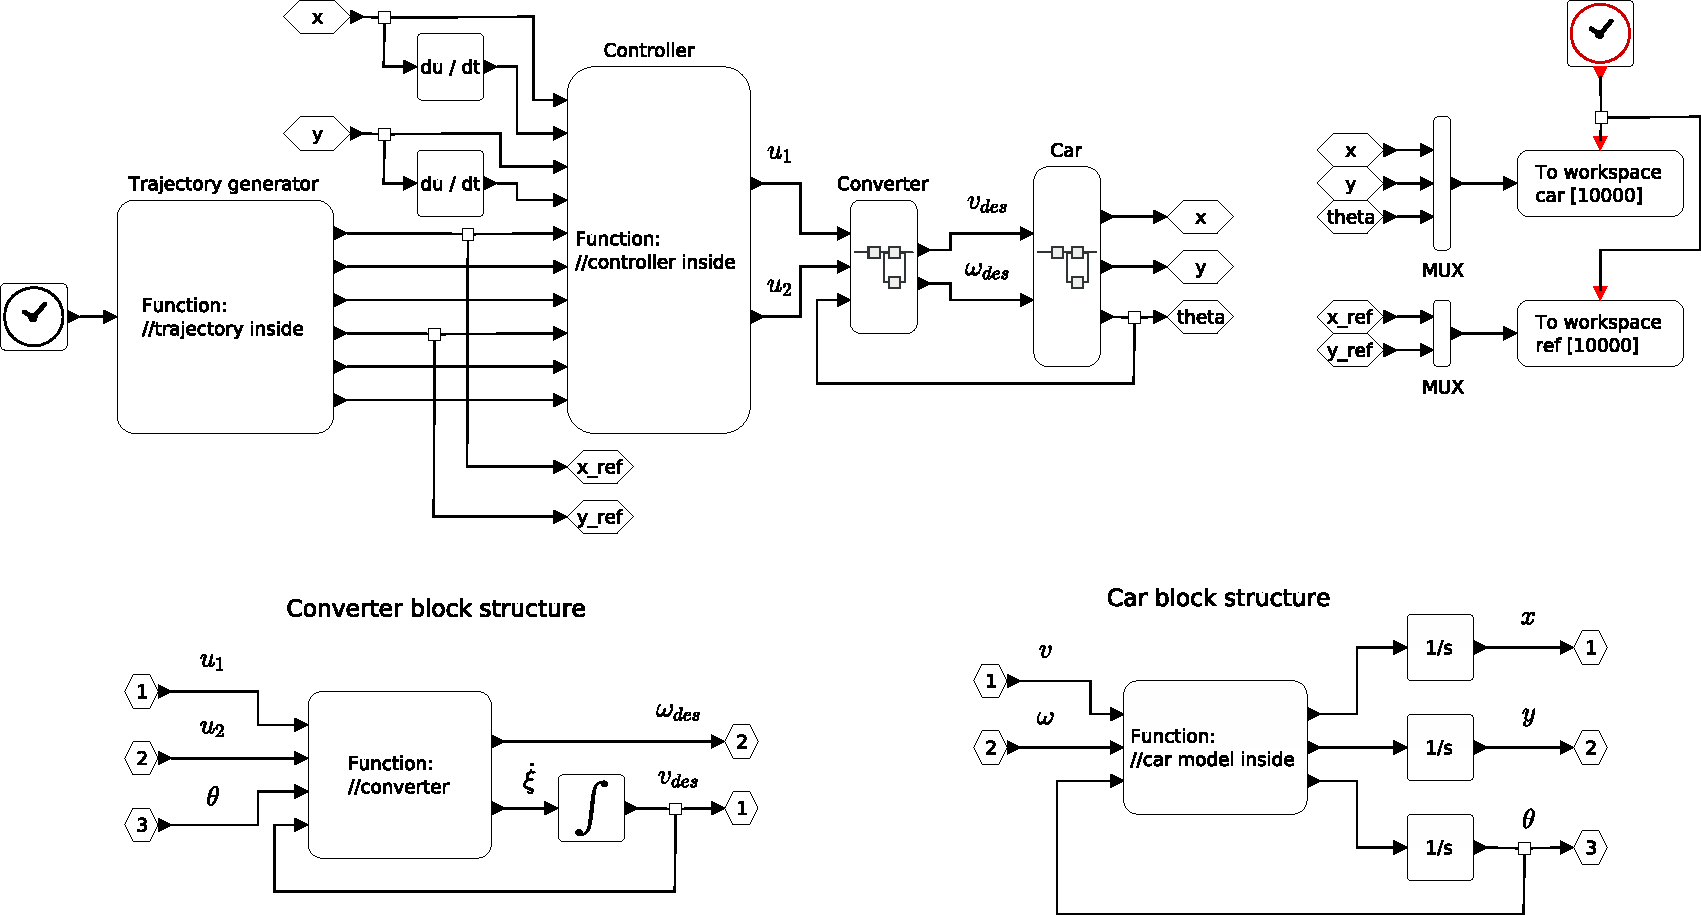
\includegraphics[width=\textwidth]{control_system_modeling_scheme.pdf}
    \vspace{0.0cm}
    \caption{Схема моделирования системы управления движением робота.}
    \label{img_control_system_modeling_scheme}
\end{figure}

\begin{figure}[h!]
    \centering
    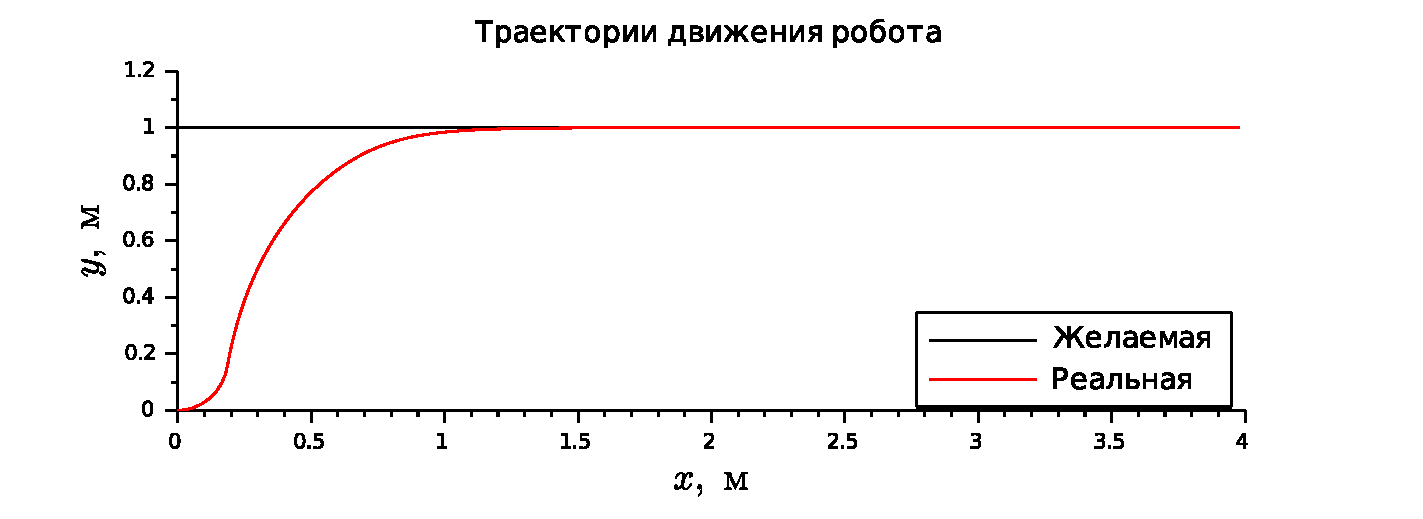
\includegraphics[width=0.9\textwidth]{simulation_trajectory.pdf}
    \vspace{0.0cm}
    \caption{Результаты запуска схемы моделирования.}
    \label{img_simulation_trajectory}
\end{figure}

\begin{figure}[h!]
    \centering
    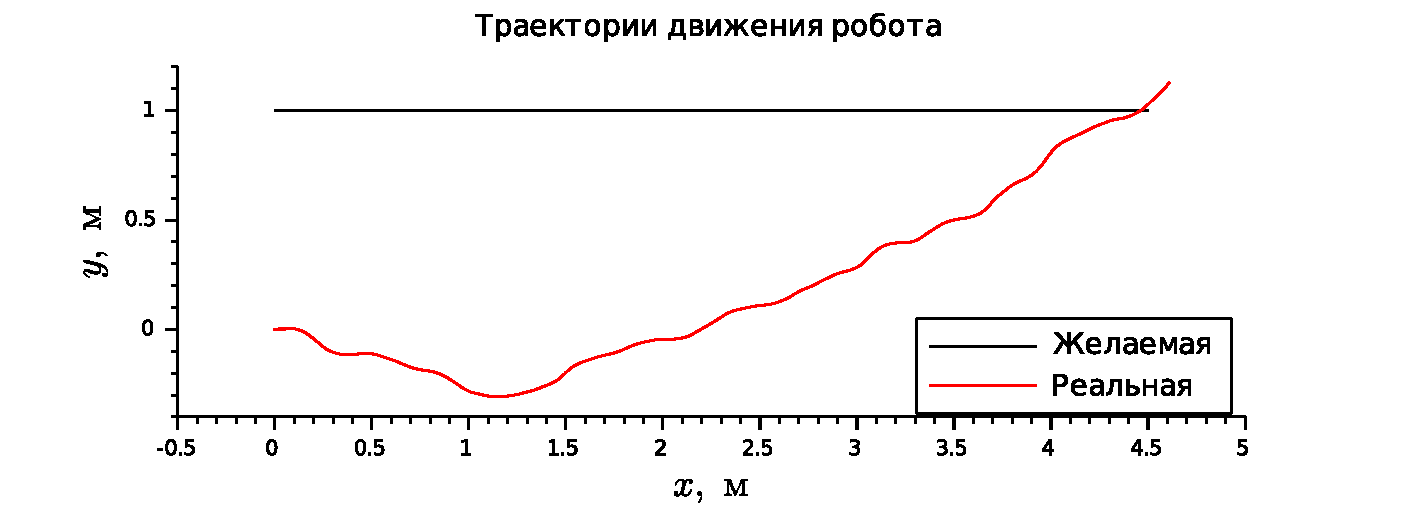
\includegraphics[width=0.9\textwidth]{movement_experiments_results.pdf}
    \vspace{0.0cm}
    \caption{Результат одного из экспериментов, проверяющего работоспособность системы управления движением.}
    \label{img_movement_experiments_results}
\end{figure}

\newpage \mbox{} \newpage \mbox{} \newpage \mbox{} \newpage